\appendix
\section{A cell-projection proof of the continuous-kernel bound}
\label{app:continuous-proof}
We prove Lemma~\ref{lem:continuous-entropy-partition}.  The steps are to replace a sample by its histogram and within-cell fluctuation, complete the square in the energy, and estimate the two resulting terms.  The histogram gives a finite-dimensional Gaussian integral; continuity makes the remaining centered kernel small.

\textbf{1. Histogram and energy projection.}
Use the partitions and box averages of Section~\ref{sec:setting}, choosing the resolution $J$ here for the fixed kernel $K$.  In the application $K=b_r$, the cutoff $r$ stays fixed while this auxiliary grid is refined.  With the corresponding labels and counts, set
\begin{equation}
 \mu_N=\frac1N\sum_i\delta_{X_i},\qquad
 f_L=\frac MN\sum_a n_a\one_{A_a},\qquad
 \nu_N=\mu_N-f_L\muunif.
 \label{eq:empirical-histogram-splitting}
\end{equation}
Thus $\nu_N(A_a)=0$.  Figure~\ref{fig:occupancy-and-offsets} shows this decomposition.

\begin{figure}[htbp]
\centering
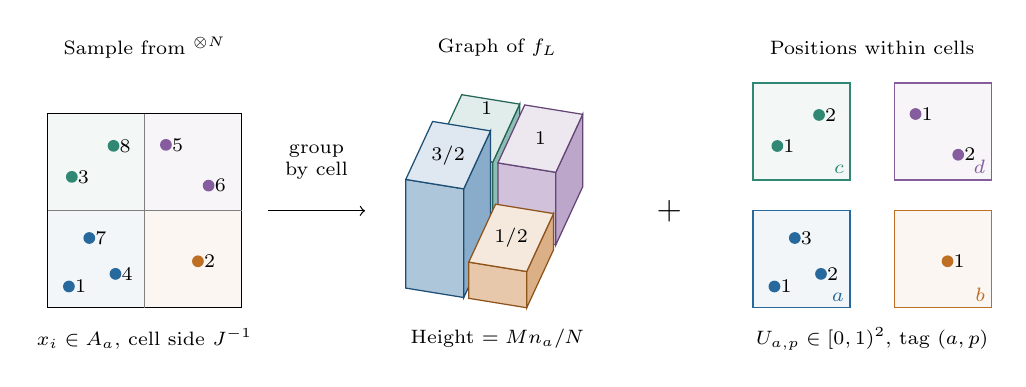
\begin{tikzpicture}[x=1.12cm,y=1.12cm,font=\scriptsize,
  particle/.style={circle,inner sep=1.5pt},
  every path/.style={line width=.45pt}]
 \definecolor{cella}{RGB}{39,104,157}
 \definecolor{cellb}{RGB}{191,111,35}
 \definecolor{cellc}{RGB}{48,135,116}
 \definecolor{celld}{RGB}{133,93,158}
 \node at (1.1,2.95) {Sample from $\muunif^{\otimes N}$};
 \node at (5.1,2.95) {Graph of $f_L$};
 \node at (9.35,2.95) {Positions within cells};
 % Original sample: four cells, eight labelled particles.
 \foreach \x/\y/\col in {0/0/cella,1.1/0/cellb,0/1.1/cellc,1.1/1.1/celld}
   \fill[\col!6] (\x,\y) rectangle +(1.1,1.1);
 \draw (0,0) rectangle (2.2,2.2);
 \draw[gray] (1.1,0)--(1.1,2.2) (0,1.1)--(2.2,1.1);
 \foreach \x/\y/\col/\id in {.242/.242/cella/1,.770/.385/cella/4,.473/.792/cella/7,1.705/.528/cellb/2,.275/1.485/cellc/3,.748/1.837/cellc/8,1.342/1.848/celld/5,1.826/1.386/celld/6} {
   \node[particle,fill=\col] at (\x,\y) {};
   \node[anchor=west,inner sep=2pt] at (\x,\y) {$\id$};
 }
 \node at (1.1,-.35) {$x_i\in A_a$, cell side $J^{-1}$};
 \draw[->] (2.5,1.1)--(3.6,1.1);
 \node[align=center] at (3.05,1.65) {group\\by cell};
 % Raised histogram: horizontal coordinates label cells, height is density.
 \begin{scope}[shift={(4.02,.20)},x={(.80cm,-.13cm)},
               y={(.37cm,.80cm)},z={(0cm,.92cm)}]
  % Draw the back row first; small gaps keep all four columns legible.
  \foreach \xx/\yy/\hh/\col in {0/1/1/cellc,1/1/1/celld,0/0/1.5/cella,1/0/.5/cellb} {
   \filldraw[fill=\col!38,draw=\col!75!black]
     (\xx+.04,\yy+.04,0)--(\xx+.96,\yy+.04,0)--
     (\xx+.96,\yy+.04,\hh)--(\xx+.04,\yy+.04,\hh)--cycle;
   \filldraw[fill=\col!55,draw=\col!75!black]
     (\xx+.96,\yy+.04,0)--(\xx+.96,\yy+.96,0)--
     (\xx+.96,\yy+.96,\hh)--(\xx+.96,\yy+.04,\hh)--cycle;
   \filldraw[fill=\col!15,draw=\col!75!black]
     (\xx+.04,\yy+.04,\hh)--(\xx+.96,\yy+.04,\hh)--
     (\xx+.96,\yy+.96,\hh)--(\xx+.04,\yy+.96,\hh)--cycle;
  }
  \node at (.5,1.82,1) {$1$};
  \node at (1.5,1.5,1) {$1$};
  \node at (.5,.5,1.5) {$3/2$};
  \node at (1.5,.5,.5) {$1/2$};
 \end{scope}
 \node at (5.1,-.35) {Height $=Mn_a/N$};
 \node[font=\large] at (7.05,1.1) {$+$};
 % Same points in four separate copies of the unit square.
 \foreach \x/\y/\col/\tag in {8/0/cella/a,9.6/0/cellb/b,8/1.45/cellc/c,9.6/1.45/celld/d} {
   \fill[\col!6] (\x,\y) rectangle +(1.1,1.1);
   \draw[\col] (\x,\y) rectangle +(1.1,1.1);
   \node[anchor=south east,inner sep=2pt,text=\col] at (\x+1.1,\y) {$\tag$};
 }
 \foreach \x/\y/\col/\id in {8.242/.242/cella/1,8.770/.385/cella/2,8.473/.792/cella/3,10.205/.528/cellb/1,8.275/1.835/cellc/1,8.748/2.187/cellc/2,9.842/2.198/celld/1,10.326/1.736/celld/2} {
   \node[particle,fill=\col] at (\x,\y) {};
   \node[anchor=west,inner sep=2pt] at (\x,\y) {$\id$};
 }
 \node at (9.35,-.35) {$U_{a,p}\in[0,1)^2$, tag $(a,p)$};
\end{tikzpicture}
\caption{A schematic with $M=4$, $N=8$.  The sample is split into its histogram $f_L$, whose column heights are the cell densities $Mn_a/N$ (height $1$ is uniform), and the positions of the particles within their cells, which carry the signed measure $\nu_N$.  Writing $x_{a,p}=J^{-1}(a+U_{a,p})$ with offsets $U_{a,p}\in[0,1)^\d$, the two right-hand panels recover the sample up to a permutation; each box on the right is a copy of the unit square, with its points numbered within that cell.  Under the uniform product law, conditional on the counts, the offsets are independent and uniform; this is the retagging used in \eqref{eq:partition-occupancy-sum}.}
\label{fig:occupancy-and-offsets}
\end{figure}


For this proof write $T=T_K$ and
$\ip{\sigma,T\tau}=\iint K(x,y)\,\dd\sigma(x)\dd\tau(y)$,
identifying a density with its measure when needed.  Continuity of $K$ makes this form finite on finite signed measures, and positivity extends from densities by approximation.  On the mean-zero cell-constant space $V_M$, define
\begin{equation}
 P_M(\nu_N)=\underset{h\in V_M}{\operatorname{argmin}}\,
                  \ip{h-\nu_N,T(h-\nu_N)}.
 \label{eq:explicit-histogram-square-shift}
\end{equation}
If the form has null directions, take the minimizer modulo them.  Cauchy--Schwarz for the nonnegative form shows that the mixed functional vanishes on these directions.  Projection orthogonality gives
\begin{equation}
 \ip{h,T(\nu_N-P_M(\nu_N))}=0
 \qquad(h\in V_M).
 \label{eq:histogram-square-shift}
\end{equation}
Put $z_N=f_L-1+P_M(\nu_N)$.  Expanding the energy and using \eqref{eq:histogram-square-shift} gives the completed square
\begin{equation}
 \begin{aligned}
 \ip{\mu_N-\muunif,T(\mu_N-\muunif)}
 &=\ip{z_N,Tz_N}+\ip{\nu_N,T\nu_N}
                   -\ip{P_M(\nu_N),TP_M(\nu_N)}\\
 &\le\ip{z_N,Tz_N}+\ip{\nu_N,T\nu_N}.
 \end{aligned}
 \label{eq:direct-square-completion}
\end{equation}

\textbf{2. Entropy bounds the completed square.}
For $h\in V_M$, the entropy variational formula and \eqref{eq:continuous-entropy-assumption} imply
\begin{equation}
 \begin{aligned}
 \log\int e^{Th}\,\dd\muunif
 &=\sup_\rho\left\{\ip{h,T(\rho-1)}-\Hr(\rho\muunif\mid\muunif)\right\}\\
 &\le\sup_\rho\left\{\ip{h,T(\rho-1)}
                         -\frac B2\ip{\rho-1,T(\rho-1)}\right\}
 \le\frac1{2B}\ip{h,Th}.
 \end{aligned}
 \label{eq:dual-log-hls}
\end{equation}
The last step completes the square in $\rho-1-h/B$.  Also, for every $h\in V_M$,
\begin{equation}
 \ip{h,Tz_N}=\int Th\,\dd\mu_N
            =\frac1N\sum_iTh(X_i),
 \label{eq:coarse-gaussian-pairing}
\end{equation}
by the definition of $\nu_N$ and projection orthogonality.

Choose coordinates on the nonnull part of $V_M$, of dimension $q_M\le M-1$, and let $\Sigma$ be the matrix of its energy form.  For a Gaussian coordinate vector $Z$ with covariance $\Sigma^{-1}$, let $\mathsf Z$ denote the corresponding cell-constant function.  The elementary identity
$\E_Z[e^{v^\top\Sigma Z}]=e^{v^\top\Sigma v/2}$ and \eqref{eq:coarse-gaussian-pairing} give, for $0\le t<B$,
\begin{equation}
 \begin{aligned}
 \E\big[e^{\frac{tN}2\ip{z_N,Tz_N}}\big]
 &=\E_Z\left[\left(\int e^{\sqrt{t/N}\,T\mathsf Z}
                           \,\dd\muunif\right)^N\right]\\
 &\le\E_Z\big[e^{\frac{t}{2B}\ip{\mathsf Z,T\mathsf Z}}\big]\\
 &=\frac1{(2\pi)^{q_M/2}\sqrt{\det(\Sigma^{-1})}}
   \int_{\R^{q_M}}e^{-\frac12(1-t/B)z^\top\Sigma z}\,\dd z\\
 &=(1-t/B)^{-q_M/2}.
 \end{aligned}
 \label{eq:coarse-partition-estimate}
\end{equation}
Here, the inequality is \eqref{eq:dual-log-hls} applied to
$h=\sqrt{t/N}\,\mathsf Z$.  Tonelli justifies exchanging the Gaussian and particle integrals.  The bound is independent of $N$ for the fixed grid.

\textbf{3. Continuity makes the remainder small.}
Set
\begin{equation}
 r_J=(I-Q_J)_x(I-Q_J)_yK.
 \label{eq:general-cell-centering}
\end{equation}
This subtracts the box average in each variable and adds back the joint average.  If $\omega_K(\varepsilon)$ is the modulus of continuity when both arguments move by at most $\varepsilon$, then
\begin{equation}
 \|r_J\|_\infty\le4\omega_K(\sqrt\d/J)\longrightarrow0.
 \label{eq:continuous-small-remainder}
\end{equation}
The kernel $r_J$ differs from $K$ by terms that are cell constant in $x$ or in $y$, and $\nu_N$ integrates cell-constant functions to zero; hence $\ip{\nu_N,T\nu_N}=\ip{\nu_N,T_{r_J}\nu_N}$.  Moreover, $r_J$ has zero average in each variable over every box, so $T_{r_J}$ annihilates the cell-constant density $f_L$, and therefore
$\ip{\nu_N,T\nu_N}=\ip{\mu_N,T_{r_J}\mu_N}=N^{-2}\sum_{i,j}r_J(X_i,X_j)$.
Removing equal particle indices in \eqref{eq:direct-square-completion}, we obtain
\begin{equation}
 \mathsf W_N(K)\le N\ip{z_N,Tz_N}
                  +\mathsf W_N(r_J)+5\|K\|_\infty.
 \label{eq:diagonal-correction-bound}
\end{equation}
Indeed, the diagonal correction is
$N^{-1}\sum_i[r_J(X_i,X_i)-K(X_i,X_i)]$, whose absolute value is at most $5\|K\|_\infty$.

Choose conjugate $p,q>1$ with $p\be_0<B$.  Since $r_J$ is centered in each variable under $\muunif$ and bounded by $\|r_J\|_\infty$, Lemma~\ref{lem:canonical-array-exponential} applies with $\kappa=\|r_J\|_\infty$ and $\theta=q\be$; by \eqref{eq:continuous-small-remainder}, a sufficiently fine fixed grid gives
$\sup_{N,\,0\le\be\le\be_0}\E[e^{q\be\mathsf W_N(r_J)/2}]\le8/3$.
H\"older and \eqref{eq:coarse-partition-estimate} now yield
\begin{equation}
 \E\big[e^{\frac\be2\mathsf W_N(K)}\big]
 \le e^{5\be_0\|K\|_\infty/2}
      (1-p\be_0/B)^{-q_M/(2p)}(8/3)^{1/q}.
 \label{eq:continuous-proof-conclusion}
\end{equation}
This proves Lemma~\ref{lem:continuous-entropy-partition}.

\begin{thebibliography}{1}
\bibitem{RenWang2025}
Z.~Ren and S.~Wang,
\emph{Size of chaos for Gibbs measures of mean field interacting diffusions},
Probability Theory and Related Fields (2025).
\href{https://doi.org/10.1007/s00440-025-01435-z}{doi:10.1007/s00440-025-01435-z}.
Accepted version: \href{https://arxiv.org/abs/2411.14236v3}{arXiv:2411.14236v3}.
\end{thebibliography}